From requirement analysis the development moves on to the design of the system and implementation.
First the functional design will be described, after that the specific decisions considering implementation are discussed.
These concern reuse of existing software, the data model, the system's architecture, and user-interface design.

Chapter 2 resulted in a compact list of requirements (figure\ref{fig:brainstorm-after}), which are now translated into functions.
An unordered list of functions can be found in appendix \ref{identified-functions}, however it is more interesting to order these functions with a workflow.
This is done according to the following research life cycle story:

\begin{quotation}
	\noindent{} A researcher wants to investigate a certain hypothesis on the \project{} dataset.
	He or she needs to register an account with the system which is then checked and approved by the data manager.
	
	Next, the researcher formulates a data request using the system.
	From the data dictionary the researcher searches (filters) for the appropriate data items (names of data items are called ``headers'').
	The researcher creates the request document with the necessary information required by the committee to decide.
	The system provides feedback based on the selected fields and automatically detected keywords.
	Based on this feedback the researcher can edit the request or send it for approval.
	Each member of the committee checks and approves the request.
	
	After approval the system creates a subset of \project{} data containing the requested data items.
	The researcher filters this subset and downloads a selection of the data.
	Another possible path is that the researcher prepares the data for analysis on the system and the outcomes are stored.
	
	To complete the request the researcher uploads the paper which is then again approved by the committee.
\end{quotation}

\noindent{}The resulting mapping between discovered functions and the research life cycle workflow is shown in figure \ref{fig:functions-workflow}.
During the brainstorm session weight was given to the requirements; therefore, functions with less priority for  implementation are displayed greyed-out (\ie{} change data, data curation, analyse, store outcomes).
Not all requirements were implemented in the final prototype - the included functions  have a dashed border.

\begin{figure}[!htb]
	\centering
	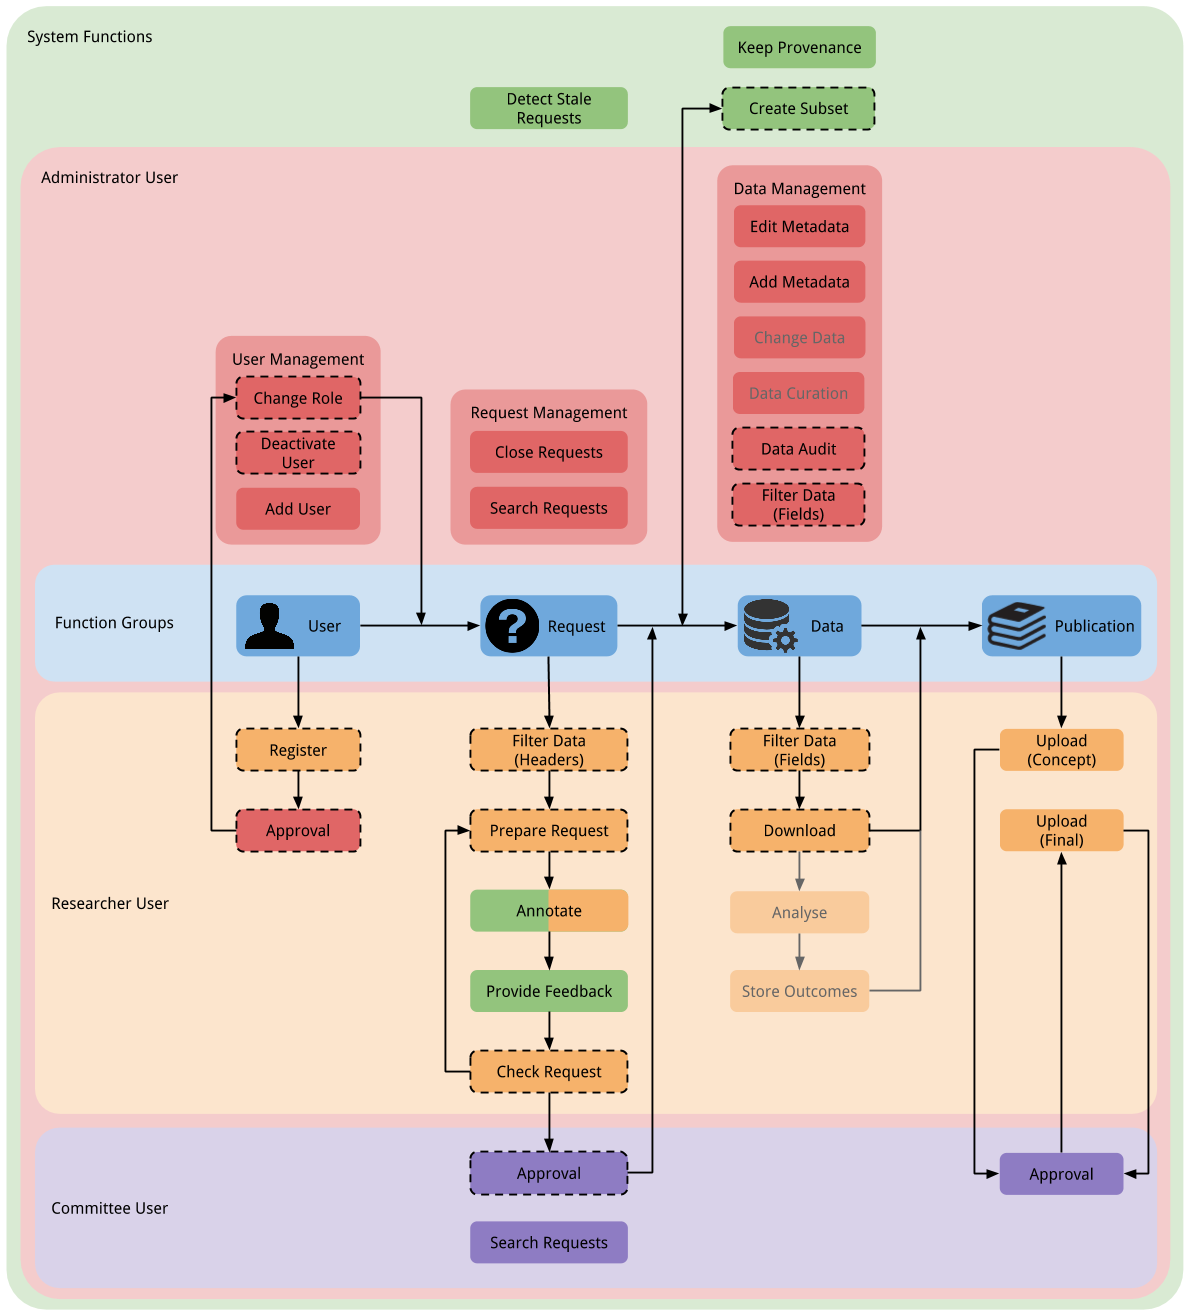
\includegraphics[width=1.0\linewidth]{images/functions-in-workflow}
	\caption{
		Gateway functions according to function groups, actors, and usage within the research workflow.
		Vertical columns represent different function groups, colours are used for different user roles, and arrows indicate sequence of actions.
		Greyed-out functions are deemed less important, which was an outcome of the brainstorm session (see section \ref{brainstorm}).
		Functions that were included in the final prototype are marked with a dashed border.
	}
	\label{fig:functions-workflow}
\end{figure}

\silvia{this figure is very important. does it belong to some subsection "functional design?" or do you think it is okay to include it in the intro}

\silvia{Need to be more explicit about the system and the prototype - the implementation does not cover the complete system, but you did consider a lot more than the actual prototype. i suggest to stick to prototype whenever you are talking about the system you implemented, just to stress that this is a small piece of a much larger scope}